%%
%% cap3.tex
%% 
%% Made by Carlos Calcaneo Roldan
%% Login   <calcaneo@jogrant>
%% 
%% Started on  Mon Jul 22 15:03:25 2019 Carlos Calcaneo Roldan
%% Last update Time-stamp: <2020-jul-29.miércoles 19:05:05 ()>
%%

\chapter{Estudió de los halos de Materia Oscura}
\setcounter{equation}{0}

%%%%%%%%EL TExto Comienza abajo de aquí! 


\section{Evolución de la cantidad de halos}

En la evolución del Universo, la materia del Universo se comenzó a agrupar lentamente en lo que llamamos halos. En un principio la materia parece una nube sin estructuras internas, mientras .,8
\begin{figure}[H]
    \centering
    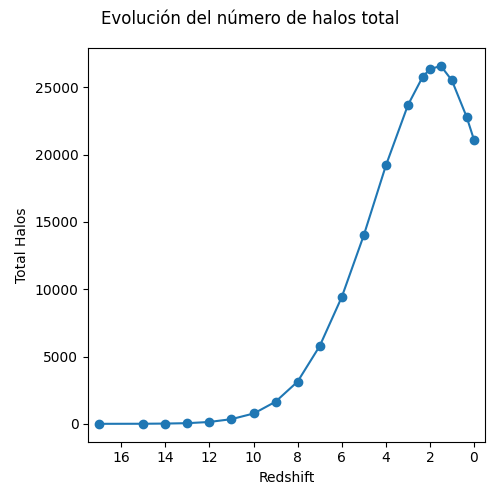
\includegraphics[scale = 0.75]{TotalHalos.png}
    \label{fig:EvoNumTotHalos}
    \caption[Evolución del Número de halos]{Se muestra el numero de halos y como cambia la cantidad conforme evoluciona el Universo en una cosmología $\Omega_\lambda = 0.691 $ y $\Omega_0 = 0.309$.}
\end{figure}


\section{Cúmulo proyectado sobre el plano de S2}


